\documentclass[hyperref={bookmarks=false},aspectratio=169]{beamer}
\usepackage[T1]{fontenc}
\usepackage[utf8]{inputenc}
\usepackage{lmodern}
\usepackage{amsmath}
\usepackage{amsfonts}
\usepackage{amssymb}
\usepackage{amsthm}
\usepackage{graphicx}
\usepackage{color}
\usepackage{xcolor}
\usepackage{url}
\usepackage{theorem}
\usepackage{textcomp}
\usepackage{listings}
\usepackage{hyperref}
\usepackage{glossaries}
\usepackage{parskip}
\usetheme{default}

\title{Arquitetura Genérica para Processamento de Eventos em Streaming utilizando Apache Kafka}
\author{Jânio Prates Otoni}
\date{\today}

\begin{document}

\begin{frame}
\titlepage
\end{frame}

%\begin{frame}
%\frametitle{}
%\begin{description}
%    \item[API] Application Programming Interface
%    \item[ROM] Read Only Memory
%    \item[RAM] Random Access Memory
%\end{description}
%\end{frame}

\begin{frame}
\frametitle{Objetivos}
\begin{itemize}
    \item Avaliar a plataforma Kafka para \textit{streaming} de dados de \textit{IoT}
    \item \textbf{NÃO} é objetivo do trabalho processar esses dados
\end{itemize}
\end{frame}

\begin{frame}
\frametitle{Referencial}
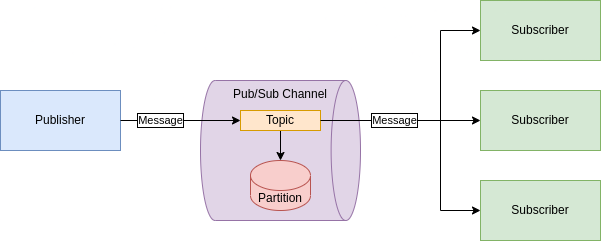
\includegraphics[scale=0.65]{imagens/pubsub.png}
\end{frame}

\begin{frame}
\frametitle{Motivação}
\begin{itemize}
    \item Sistema de Internet das Coisas para Detecção de Incêndios Florestais
    \item Formato de Dados
    \begin{itemize}
        \item Avro é amplamente utilizado em \textit{big data}
        \item Programas lêm e processam binários com mais facilidade
        \item Formatos binários são mais compactos
        \item Avro obriga a utilização de esquemas para a definição dos dados
    \end{itemize}
\end{itemize}
\end{frame}

\begin{frame}
\frametitle{Trabalhos Relacionados}
\begin{itemize}
    \item   Albuquerque, S., Fonseca, D., Lima, R. L., Milanés, A., Rocha, I., Santos, A. M., Silva, G., and Vieira, F. (2020). Sistema de internet das coisas para detecção de incêndios florestais. In Anais do XI Workshop de Computação Aplicada à Gestão do Meio Ambiente e Recursos Naturais, pages 141–150. SBC.
    \item   Albuquerque, S., Silva, F., and Oliveira, D. (2021). Análise espacial da distribuição de sensores para detecção de incêndios florestais no parque estadual da serra do rola moça. In Anais do XII Workshop de Computação Aplicada à Gestão do Meio Ambiente e Recursos Naturais, pages 11–18, Porto Alegre, RS, Brasil. SBC.
    \item   Mishra, B., Mishra, B., and Kertesz, A. (2021). Stress-testing mqtt brokers: A comparative analysis of performance measurements. Energies, 14(18):5817.
\end{itemize}
\end{frame}

\begin{frame}
\frametitle{Fluxo de Dados}
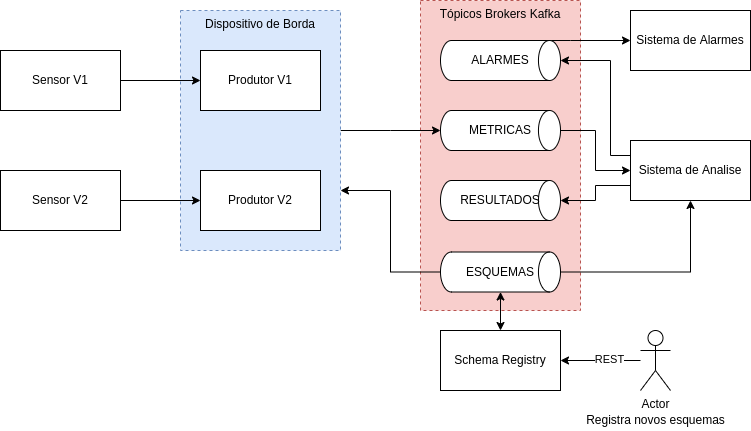
\includegraphics[scale=0.5]{imagens/fluxo_de_dados.png}
\end{frame}

\begin{frame}
\frametitle{Experimentos}
Quatro máquinas virtuais com:
\begin{itemize} 
    \item 1 vCPU ARM; 
    \item 6 GB de memória RAM; 
    \item 1 vNIC com 1 Gigabit Ethernet. 
\end{itemize} 
\begin{table}[ht] 
\caption{Quantidade de mensagens por segundo e uso percentual de CPU relacionado ou número de produtores em execução}
\centering 
    \begin{tabular}{ |c|c|c|c|c|c|c|c|c| } 
        \hline 
        Produtores  & 1     & 2     & 3     & 4         & 5         & 6         & 7         & 8         \\
        \hline 
        msg/seg     & 808   & 1622  & 2260  & 2915      & 3624      & 4383      & 4876      & 5632      \\
        \% CPU      & 96.35 & 99.80 & 99.68 & 100.00    & 100.00    & 100.00    & 100.00    & 100.00    \\ 
        \hline 
    \end{tabular} 
    \label{tab:uso_recursos_caso_base} 
\end{table}
\end{frame}

\begin{frame}
\frametitle{Número de Mensagens Produzidas em Cada Configuração do Cluster}
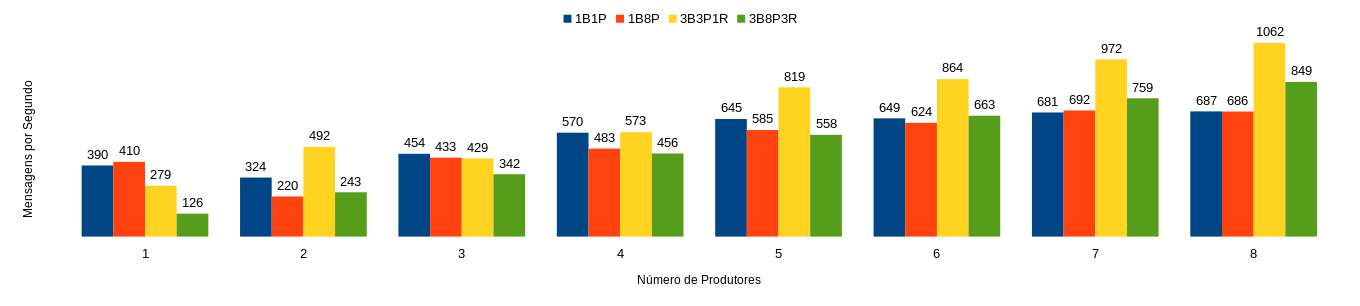
\includegraphics[scale=0.3]{imagens/mensagens_por_segundo.png}
\begin{description}
    \item[1B1P] 1 \textit{broker} e 1 partição
    \item[1B8P] 1 \textit{broker} e 8 partições
    \item[3B3P1R] 3 \textit{brokers}, 3 partições e 1 réplica
    \item[3B8P3R] 3 \textit{brokers}, 8 partições e 3 réplicas
\end{description}
\end{frame}

\begin{frame}
\frametitle{Uso de CPU em Cada Configuração do Cluster}
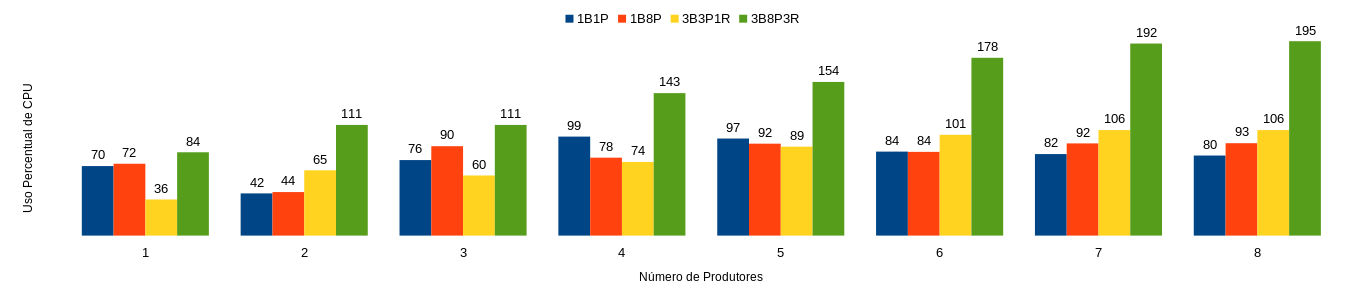
\includegraphics[scale=0.3]{imagens/uso_de_cpu.png}
\end{frame}

\begin{frame}
\frametitle{Conclusões e Trabalhos Futuros}
\begin{itemize}
    \item Oferece maior flexibilidade e uma quantidade maior de dados a serem trafegados
    \item Dependendo da escala, podem ser utilizados Raspberry Pi 4 Model B (4GB)
    \item Pode Pode ser utilizado para análise de dados com baixa latência
\end{itemize}
\end{frame}

\end{document}